% Fig. 2（fig:overview）：(a) 參數化、(b) 色彩旋轉、(c) 最佳化。
% 編譯：先以 docs/paper_tools/generate_method_overview_panels.py 產生 lattice_*.tex、disk_*.tex、disk_background.png
%（遠端執行，輸出複製到本目錄），再於本目錄執行 tectonic -X compile method_overview.tex，
% 把 method_overview.pdf 複製到 docs/paper/fig/。
% (a) 與 (b) 左側球帽為示意；(b) 右側色度盤為 woman_00、color3d 的實際 LUT。
\documentclass[tikz,border=1pt]{standalone}
\usepackage{amsmath,amssymb,mathptmx}
\usepackage[no-math]{fontspec}
\setmainfont{texgyretermes}[Extension=.otf, UprightFont=*-regular, BoldFont=*-bold, ItalicFont=*-italic, BoldItalicFont=*-bolditalic]
\usetikzlibrary{calc,arrows.meta}

\definecolor{ink}{HTML}{111111}
\definecolor{muted}{HTML}{7A7A7A}
\definecolor{panel}{HTML}{F4F4F4}
\definecolor{ours}{HTML}{1F6F7C}
\definecolor{polar}{HTML}{2F5DA8}
\definecolor{azim}{HTML}{C9781A}

\tikzset{
  >={Stealth[length=4.5pt,width=3.4pt]},
  lattice/.style={black!30, line width=0.3pt},
  node/.style={black!55},
  vec/.style={-{Stealth[length=2.3pt,width=1.8pt]}, black!72, line width=0.35pt},
  disp/.style={-{Stealth[length=2.2pt,width=1.9pt]}, black!62, line width=0.5pt},
  flow/.style={->, ink, line width=0.8pt},
  grad/.style={->, ours, densely dashed, line width=0.8pt},
  title/.style={anchor=north west, font=\small\bfseries, inner sep=0pt},
  lab/.style={font=\footnotesize, inner sep=1.5pt},
  small/.style={font=\scriptsize, inner sep=1.5pt, text=muted},
}
\newcommand{\pixelring}[2]{\draw[white, line width=1.8pt] (#1) circle (2.1pt);\draw[#2, line width=0.9pt] (#1) circle (2.1pt);}

% 區塊邊界（cm）
\def\aR{4.0}\def\bL{4.15}\def\bR{11.55}\def\cL{11.7}\def\W{17.4}\def\H{6.45}

% (b) 球帽示意：球心 (bx, by)，半徑 \Rs，視角仰角 \Elev；θ 自灰軸量起，φ 繞灰軸
\def\bx{6.25}\def\by{0.62}\def\Rs{2.6}\def\Elev{28}
\tikzset{cap/.cd, t/.store in=\capt, p/.store in=\capp}
\tikzdeclarecoordinatesystem{cap}{\tikzset{cap/.cd,#1}%
  \pgfmathsetmacro{\cpx}{\bx+\Rs*sin(\capt)*cos(\capp)}%
  \pgfmathsetmacro{\cpy}{\by+\Rs*cos(\capt)*cos(\Elev)+\Rs*sin(\capt)*sin(\capp)*sin(\Elev)}%
  \pgfpointxy{\cpx}{\cpy}}
% c 與 c′（示意位置）
\def\tC{42}\def\pC{232}\def\tN{29}\def\pN{257}

\begin{document}
\begin{tikzpicture}[line cap=round]

% ---- 三個區塊 ----
\fill[panel, rounded corners=3pt] (0,0) rectangle (\aR,\H);
\fill[panel, rounded corners=3pt] (\bL,0) rectangle (\bR,\H);
\fill[panel, rounded corners=3pt] (\cL,0) rectangle (\W,\H);
\node[title] at (0.2,\H-0.2) {(a) Parameterization};
\node[title] at (\bL+0.2,\H-0.2) {(b) Color rotation};
\node[title] at (\cL+0.2,\H-0.2) {(c) Optimization};

% ======== (a)：Θ → G_σ → V ========
\begin{scope}[shift={(2.0,4.4)}, scale=1.25]\draw[lattice] (0.000,0.000) -- (-0.620,-0.360);
\draw[lattice] (0.000,0.000) -- (0.620,-0.360);
\draw[lattice] (0.000,0.000) -- (0.000,0.720);
\draw[lattice] (-0.620,-0.360) -- (0.000,-0.720);
\draw[lattice] (-0.620,-0.360) -- (-0.620,0.360);
\draw[lattice] (0.620,-0.360) -- (0.000,-0.720);
\draw[lattice] (0.620,-0.360) -- (0.620,0.360);
\draw[lattice] (0.000,0.720) -- (-0.620,0.360);
\draw[lattice] (0.000,0.720) -- (0.620,0.360);
\draw[lattice] (0.000,-0.720) -- (0.000,0.000);
\draw[lattice] (-0.620,0.360) -- (0.000,0.000);
\draw[lattice] (0.620,0.360) -- (0.000,0.000);
\fill[node] (0.000,0.720) circle (0.45pt);
\draw[vec] (0.000,0.720) -- ++(0.027,0.037);
\fill[node] (0.155,0.630) circle (0.45pt);
\draw[vec] (0.155,0.630) -- ++(-0.002,0.017);
\fill[node] (-0.155,0.630) circle (0.45pt);
\draw[vec] (-0.155,0.630) -- ++(0.058,0.001);
\fill[node] (0.310,0.540) circle (0.45pt);
\draw[vec] (0.310,0.540) -- ++(0.086,-0.011);
\fill[node] (0.000,0.540) circle (0.45pt);
\draw[vec] (0.000,0.540) -- ++(0.108,-0.052);
\fill[node] (-0.310,0.540) circle (0.45pt);
\draw[vec] (-0.310,0.540) -- ++(-0.026,0.007);
\fill[node] (0.465,0.450) circle (0.45pt);
\draw[vec] (0.465,0.450) -- ++(0.038,0.143);
\fill[node] (0.155,0.450) circle (0.45pt);
\draw[vec] (0.155,0.450) -- ++(0.087,-0.073);
\fill[node] (-0.155,0.450) circle (0.45pt);
\draw[vec] (-0.155,0.450) -- ++(-0.024,0.126);
\fill[node] (-0.465,0.450) circle (0.45pt);
\draw[vec] (-0.465,0.450) -- ++(-0.107,-0.077);
\fill[node] (0.620,0.360) circle (0.45pt);
\draw[vec] (0.620,0.360) -- ++(-0.014,-0.059);
\fill[node] (0.310,0.360) circle (0.45pt);
\draw[vec] (0.310,0.360) -- ++(0.010,-0.079);
\fill[node] (0.000,0.360) circle (0.45pt);
\draw[vec] (0.000,0.360) -- ++(0.070,-0.078);
\fill[node] (-0.310,0.360) circle (0.45pt);
\draw[vec] (-0.310,0.360) -- ++(-0.005,-0.028);
\fill[node] (-0.620,0.360) circle (0.45pt);
\draw[vec] (-0.620,0.360) -- ++(-0.058,-0.085);
\fill[node] (0.620,0.180) circle (0.45pt);
\draw[vec] (0.620,0.180) -- ++(0.048,-0.040);
\fill[node] (0.465,0.270) circle (0.45pt);
\draw[vec] (0.465,0.270) -- ++(-0.077,-0.053);
\fill[node] (0.155,0.270) circle (0.45pt);
\draw[vec] (0.155,0.270) -- ++(-0.028,-0.113);
\fill[node] (-0.155,0.270) circle (0.45pt);
\draw[vec] (-0.155,0.270) -- ++(0.007,-0.008);
\fill[node] (-0.620,0.180) circle (0.45pt);
\draw[vec] (-0.620,0.180) -- ++(-0.030,-0.083);
\fill[node] (-0.465,0.270) circle (0.45pt);
\draw[vec] (-0.465,0.270) -- ++(-0.082,-0.003);
\fill[node] (0.620,0.000) circle (0.45pt);
\draw[vec] (0.620,0.000) -- ++(0.010,-0.066);
\fill[node] (0.465,0.090) circle (0.45pt);
\draw[vec] (0.465,0.090) -- ++(0.023,-0.029);
\fill[node] (0.310,0.180) circle (0.45pt);
\draw[vec] (0.310,0.180) -- ++(0.144,0.003);
\fill[node] (0.000,0.180) circle (0.45pt);
\draw[vec] (0.000,0.180) -- ++(-0.013,-0.174);
\fill[node] (-0.620,0.000) circle (0.45pt);
\draw[vec] (-0.620,0.000) -- ++(0.034,0.088);
\fill[node] (-0.465,0.090) circle (0.45pt);
\draw[vec] (-0.465,0.090) -- ++(-0.001,-0.032);
\fill[node] (-0.310,0.180) circle (0.45pt);
\draw[vec] (-0.310,0.180) -- ++(-0.103,-0.100);
\fill[node] (0.620,-0.180) circle (0.45pt);
\draw[vec] (0.620,-0.180) -- ++(-0.078,0.089);
\fill[node] (0.465,-0.090) circle (0.45pt);
\draw[vec] (0.465,-0.090) -- ++(-0.070,-0.011);
\fill[node] (0.310,-0.000) circle (0.45pt);
\draw[vec] (0.310,-0.000) -- ++(0.086,0.098);
\fill[node] (0.155,0.090) circle (0.45pt);
\draw[vec] (0.155,0.090) -- ++(-0.011,0.073);
\fill[node] (-0.620,-0.180) circle (0.45pt);
\draw[vec] (-0.620,-0.180) -- ++(0.063,-0.070);
\fill[node] (-0.465,-0.090) circle (0.45pt);
\draw[vec] (-0.465,-0.090) -- ++(0.062,0.042);
\fill[node] (-0.310,-0.000) circle (0.45pt);
\draw[vec] (-0.310,-0.000) -- ++(0.048,0.125);
\fill[node] (-0.155,0.090) circle (0.45pt);
\draw[vec] (-0.155,0.090) -- ++(-0.188,-0.016);
\fill[node] (0.620,-0.360) circle (0.45pt);
\draw[vec] (0.620,-0.360) -- ++(0.052,0.028);
\fill[node] (0.465,-0.270) circle (0.45pt);
\draw[vec] (0.465,-0.270) -- ++(0.090,-0.027);
\fill[node] (0.310,-0.180) circle (0.45pt);
\draw[vec] (0.310,-0.180) -- ++(-0.028,-0.049);
\fill[node] (0.155,-0.090) circle (0.45pt);
\draw[vec] (0.155,-0.090) -- ++(-0.049,0.046);
\fill[node] (-0.620,-0.360) circle (0.45pt);
\draw[vec] (-0.620,-0.360) -- ++(0.007,0.043);
\fill[node] (-0.465,-0.270) circle (0.45pt);
\draw[vec] (-0.465,-0.270) -- ++(0.035,0.013);
\fill[node] (-0.310,-0.180) circle (0.45pt);
\draw[vec] (-0.310,-0.180) -- ++(0.083,0.007);
\fill[node] (-0.155,-0.090) circle (0.45pt);
\draw[vec] (-0.155,-0.090) -- ++(-0.060,-0.059);
\fill[node] (0.000,0.000) circle (0.45pt);
\draw[vec] (0.000,0.000) -- ++(-0.049,-0.055);
\fill[node] (0.465,-0.450) circle (0.45pt);
\draw[vec] (0.465,-0.450) -- ++(0.020,0.052);
\fill[node] (0.310,-0.360) circle (0.45pt);
\draw[vec] (0.310,-0.360) -- ++(0.004,0.015);
\fill[node] (0.155,-0.270) circle (0.45pt);
\draw[vec] (0.155,-0.270) -- ++(0.049,-0.007);
\fill[node] (-0.465,-0.450) circle (0.45pt);
\draw[vec] (-0.465,-0.450) -- ++(-0.136,-0.033);
\fill[node] (-0.310,-0.360) circle (0.45pt);
\draw[vec] (-0.310,-0.360) -- ++(0.023,0.024);
\fill[node] (-0.155,-0.270) circle (0.45pt);
\draw[vec] (-0.155,-0.270) -- ++(0.030,-0.078);
\fill[node] (0.000,-0.180) circle (0.45pt);
\draw[vec] (0.000,-0.180) -- ++(0.057,-0.021);
\fill[node] (0.310,-0.540) circle (0.45pt);
\draw[vec] (0.310,-0.540) -- ++(-0.033,-0.057);
\fill[node] (0.155,-0.450) circle (0.45pt);
\draw[vec] (0.155,-0.450) -- ++(-0.030,0.078);
\fill[node] (-0.310,-0.540) circle (0.45pt);
\draw[vec] (-0.310,-0.540) -- ++(-0.194,-0.026);
\fill[node] (-0.155,-0.450) circle (0.45pt);
\draw[vec] (-0.155,-0.450) -- ++(-0.055,0.013);
\fill[node] (0.000,-0.360) circle (0.45pt);
\draw[vec] (0.000,-0.360) -- ++(0.023,0.013);
\fill[node] (0.155,-0.630) circle (0.45pt);
\draw[vec] (0.155,-0.630) -- ++(-0.039,-0.083);
\fill[node] (-0.155,-0.630) circle (0.45pt);
\draw[vec] (-0.155,-0.630) -- ++(-0.096,0.016);
\fill[node] (0.000,-0.540) circle (0.45pt);
\draw[vec] (0.000,-0.540) -- ++(-0.009,0.135);
\fill[node] (0.000,-0.720) circle (0.45pt);
\draw[vec] (0.000,-0.720) -- ++(0.041,-0.014);
\end{scope}
\node[lab, anchor=west] at (3.0,4.85) {$\Theta$};
\node[small, anchor=north] at (2.0,3.42) {free vectors on $33^3$ nodes};
\draw[flow] (2.0,3.0) -- (2.0,2.55);
\node[lab, anchor=west] at (2.12,2.78) {$G_\sigma$, $\sigma=4$ cells};
\begin{scope}[shift={(2.0,1.42)}, scale=1.25]\draw[lattice] (0.000,0.000) -- (-0.620,-0.360);
\draw[lattice] (0.000,0.000) -- (0.620,-0.360);
\draw[lattice] (0.000,0.000) -- (0.000,0.720);
\draw[lattice] (-0.620,-0.360) -- (0.000,-0.720);
\draw[lattice] (-0.620,-0.360) -- (-0.620,0.360);
\draw[lattice] (0.620,-0.360) -- (0.000,-0.720);
\draw[lattice] (0.620,-0.360) -- (0.620,0.360);
\draw[lattice] (0.000,0.720) -- (-0.620,0.360);
\draw[lattice] (0.000,0.720) -- (0.620,0.360);
\draw[lattice] (0.000,-0.720) -- (0.000,0.000);
\draw[lattice] (-0.620,0.360) -- (0.000,0.000);
\draw[lattice] (0.620,0.360) -- (0.000,0.000);
\fill[node] (0.000,0.720) circle (0.45pt);
\draw[vec] (0.000,0.720) -- ++(-0.027,-0.022);
\fill[node] (0.155,0.630) circle (0.45pt);
\draw[vec] (0.155,0.630) -- ++(-0.018,-0.048);
\fill[node] (-0.155,0.630) circle (0.45pt);
\draw[vec] (-0.155,0.630) -- ++(-0.016,-0.028);
\fill[node] (0.310,0.540) circle (0.45pt);
\draw[vec] (0.310,0.540) -- ++(0.018,-0.051);
\fill[node] (0.000,0.540) circle (0.45pt);
\draw[vec] (0.000,0.540) -- ++(-0.007,-0.061);
\fill[node] (-0.310,0.540) circle (0.45pt);
\draw[vec] (-0.310,0.540) -- ++(-0.022,-0.028);
\fill[node] (0.465,0.450) circle (0.45pt);
\draw[vec] (0.465,0.450) -- ++(0.055,-0.037);
\fill[node] (0.155,0.450) circle (0.45pt);
\draw[vec] (0.155,0.450) -- ++(0.026,-0.072);
\fill[node] (-0.155,0.450) circle (0.45pt);
\draw[vec] (-0.155,0.450) -- ++(-0.017,-0.068);
\fill[node] (-0.465,0.450) circle (0.45pt);
\draw[vec] (-0.465,0.450) -- ++(-0.038,-0.021);
\fill[node] (0.620,0.360) circle (0.45pt);
\draw[vec] (0.620,0.360) -- ++(0.072,-0.018);
\fill[node] (0.310,0.360) circle (0.45pt);
\draw[vec] (0.310,0.360) -- ++(0.057,-0.061);
\fill[node] (0.000,0.360) circle (0.45pt);
\draw[vec] (0.000,0.360) -- ++(0.008,-0.092);
\fill[node] (-0.310,0.360) circle (0.45pt);
\draw[vec] (-0.310,0.360) -- ++(-0.040,-0.069);
\fill[node] (-0.620,0.360) circle (0.45pt);
\draw[vec] (-0.620,0.360) -- ++(-0.056,-0.013);
\fill[node] (0.620,0.180) circle (0.45pt);
\draw[vec] (0.620,0.180) -- ++(0.097,-0.023);
\fill[node] (0.465,0.270) circle (0.45pt);
\draw[vec] (0.465,0.270) -- ++(0.068,-0.039);
\fill[node] (0.155,0.270) circle (0.45pt);
\draw[vec] (0.155,0.270) -- ++(0.032,-0.091);
\fill[node] (-0.155,0.270) circle (0.45pt);
\draw[vec] (-0.155,0.270) -- ++(-0.027,-0.106);
\fill[node] (-0.620,0.180) circle (0.45pt);
\draw[vec] (-0.620,0.180) -- ++(-0.059,0.018);
\fill[node] (-0.465,0.270) circle (0.45pt);
\draw[vec] (-0.465,0.270) -- ++(-0.064,-0.063);
\fill[node] (0.620,0.000) circle (0.45pt);
\draw[vec] (0.620,0.000) -- ++(0.099,-0.036);
\fill[node] (0.465,0.090) circle (0.45pt);
\draw[vec] (0.465,0.090) -- ++(0.098,-0.033);
\fill[node] (0.310,0.180) circle (0.45pt);
\draw[vec] (0.310,0.180) -- ++(0.038,-0.072);
\fill[node] (0.000,0.180) circle (0.45pt);
\draw[vec] (0.000,0.180) -- ++(-0.013,-0.120);
\fill[node] (-0.620,0.000) circle (0.45pt);
\draw[vec] (-0.620,0.000) -- ++(-0.081,0.054);
\fill[node] (-0.465,0.090) circle (0.45pt);
\draw[vec] (-0.465,0.090) -- ++(-0.049,-0.022);
\fill[node] (-0.310,0.180) circle (0.45pt);
\draw[vec] (-0.310,0.180) -- ++(-0.062,-0.110);
\fill[node] (0.620,-0.180) circle (0.45pt);
\draw[vec] (0.620,-0.180) -- ++(0.072,-0.048);
\fill[node] (0.465,-0.090) circle (0.45pt);
\draw[vec] (0.465,-0.090) -- ++(0.100,-0.033);
\fill[node] (0.310,-0.000) circle (0.45pt);
\draw[vec] (0.310,-0.000) -- ++(0.067,-0.057);
\fill[node] (0.155,0.090) circle (0.45pt);
\draw[vec] (0.155,0.090) -- ++(-0.014,-0.109);
\fill[node] (-0.620,-0.180) circle (0.45pt);
\draw[vec] (-0.620,-0.180) -- ++(-0.117,0.076);
\fill[node] (-0.465,-0.090) circle (0.45pt);
\draw[vec] (-0.465,-0.090) -- ++(-0.059,0.030);
\fill[node] (-0.310,-0.000) circle (0.45pt);
\draw[vec] (-0.310,-0.000) -- ++(-0.034,-0.063);
\fill[node] (-0.155,0.090) circle (0.45pt);
\draw[vec] (-0.155,0.090) -- ++(-0.061,-0.135);
\fill[node] (0.620,-0.360) circle (0.45pt);
\draw[vec] (0.620,-0.360) -- ++(0.027,-0.044);
\fill[node] (0.465,-0.270) circle (0.45pt);
\draw[vec] (0.465,-0.270) -- ++(0.070,-0.033);
\fill[node] (0.310,-0.180) circle (0.45pt);
\draw[vec] (0.310,-0.180) -- ++(0.066,-0.041);
\fill[node] (0.155,-0.090) circle (0.45pt);
\draw[vec] (0.155,-0.090) -- ++(0.009,-0.085);
\fill[node] (-0.620,-0.360) circle (0.45pt);
\draw[vec] (-0.620,-0.360) -- ++(-0.153,0.077);
\fill[node] (-0.465,-0.270) circle (0.45pt);
\draw[vec] (-0.465,-0.270) -- ++(-0.095,0.069);
\fill[node] (-0.310,-0.180) circle (0.45pt);
\draw[vec] (-0.310,-0.180) -- ++(-0.036,-0.003);
\fill[node] (-0.155,-0.090) circle (0.45pt);
\draw[vec] (-0.155,-0.090) -- ++(-0.034,-0.093);
\fill[node] (0.000,0.000) circle (0.45pt);
\draw[vec] (0.000,0.000) -- ++(-0.070,-0.132);
\fill[node] (0.465,-0.450) circle (0.45pt);
\draw[vec] (0.465,-0.450) -- ++(0.021,-0.026);
\fill[node] (0.310,-0.360) circle (0.45pt);
\draw[vec] (0.310,-0.360) -- ++(0.030,-0.026);
\fill[node] (0.155,-0.270) circle (0.45pt);
\draw[vec] (0.155,-0.270) -- ++(0.003,-0.055);
\fill[node] (-0.465,-0.450) circle (0.45pt);
\draw[vec] (-0.465,-0.450) -- ++(-0.143,0.083);
\fill[node] (-0.310,-0.360) circle (0.45pt);
\draw[vec] (-0.310,-0.360) -- ++(-0.071,0.047);
\fill[node] (-0.155,-0.270) circle (0.45pt);
\draw[vec] (-0.155,-0.270) -- ++(-0.035,-0.038);
\fill[node] (0.000,-0.180) circle (0.45pt);
\draw[vec] (0.000,-0.180) -- ++(-0.057,-0.105);
\fill[node] (0.310,-0.540) circle (0.45pt);
\draw[vec] (0.310,-0.540) -- ++(-0.020,-0.015);
\fill[node] (0.155,-0.450) circle (0.45pt);
\draw[vec] (0.155,-0.450) -- ++(-0.035,-0.026);
\fill[node] (-0.310,-0.540) circle (0.45pt);
\draw[vec] (-0.310,-0.540) -- ++(-0.126,0.068);
\fill[node] (-0.155,-0.450) circle (0.45pt);
\draw[vec] (-0.155,-0.450) -- ++(-0.070,0.009);
\fill[node] (0.000,-0.360) circle (0.45pt);
\draw[vec] (0.000,-0.360) -- ++(-0.067,-0.066);
\fill[node] (0.155,-0.630) circle (0.45pt);
\draw[vec] (0.155,-0.630) -- ++(-0.081,-0.010);
\fill[node] (-0.155,-0.630) circle (0.45pt);
\draw[vec] (-0.155,-0.630) -- ++(-0.119,0.032);
\fill[node] (0.000,-0.540) circle (0.45pt);
\draw[vec] (0.000,-0.540) -- ++(-0.101,-0.029);
\fill[node] (0.000,-0.720) circle (0.45pt);
\draw[vec] (0.000,-0.720) -- ++(-0.137,-0.008);
\end{scope}
\node[lab, anchor=west] at (3.0,1.87) {$V$};
\node[small, anchor=north] at (2.0,0.44) {smooth field $V=G_\sigma*\Theta$};
\draw[grad] (0.35,5.55) -- (0.95,5.05);
\node[lab, text=ours, anchor=south] at (0.35,5.52) {$\nabla_\Theta$};

% ======== (b) 左：球帽上的一個顏色 ========
\draw[muted, densely dashed, line width=0.5pt] (\bx,\by) -- (cap cs:t=0,p=0);
\foreach \t in {16,32,48}{
  \draw[black!28, line width=0.4pt] plot[domain=180:360, samples=40, smooth, variable=\p] (cap cs:t=\t,p=\p);
  \draw[black!13, line width=0.4pt] plot[domain=0:180, samples=40, smooth, variable=\p] (cap cs:t=\t,p=\p);
}
\foreach \p in {200,230,...,350}{
  \draw[black!28, line width=0.4pt] plot[domain=0:48, samples=20, smooth, variable=\t] (cap cs:t=\t,p=\p);
}
\draw[->, muted, line width=0.5pt] (cap cs:t=0,p=0) -- ++(0,0.6) node[small, above] {gray axis};
\fill[muted] (cap cs:t=0,p=0) circle (1.1pt);
\draw[black!40, line width=0.45pt] (\bx,\by) -- (cap cs:t=\tC,p=\pC);
\draw[black!40, line width=0.45pt] (\bx,\by) -- (cap cs:t=\tN,p=\pN);
\fill[black] (\bx,\by) circle (1.4pt);
\node[small, anchor=north] at (\bx,\by-0.04) {black};
\node[small, anchor=east] at ($(\bx,\by)!0.45!(cap cs:t=\tC,p=\pC)+(-0.08,0)$) {$\|c'\|=\|c\|$};

% c 處的切向量：V(c) 分解成 v_θ e_θ（沿經線）與 v_φ e_φ（沿緯圈）
\coordinate (C) at (cap cs:t=\tC,p=\pC);
% 有界後的移動（寬淡色帶）：先 Δθ 再 Δφ
\draw[polar, line width=3.6pt, opacity=0.45] plot[domain=\tC:\tN, samples=15, smooth, variable=\t] (cap cs:t=\t,p=\pC);
\draw[azim, line width=3.6pt, opacity=0.5] plot[domain=\pC:\pN, samples=15, smooth, variable=\p] (cap cs:t=\tN,p=\p);

\coordinate (Tt) at ($(C)!1.0!(cap cs:t=\tC-24,p=\pC)$);
\coordinate (Tp) at ($(C)!1.0!(cap cs:t=\tC,p=\pC+62)$);
\coordinate (TV) at ($(Tt)+(Tp)-(C)$);
\draw[black!45, densely dotted, line width=0.5pt] (Tt) -- (TV) -- (Tp);
\draw[->, polar, line width=1.1pt] (C) -- (Tt);
\draw[->, azim, line width=1.1pt] (C) -- (Tp);
\draw[->, ink, line width=0.9pt] (C) -- (TV);
\node[lab, polar, anchor=east] at ($(Tt)+(-0.08,-0.12)$) {$v_\theta e_\theta$};
\node[lab, azim, anchor=north west] at ($(Tp)+(-0.25,-0.04)$) {$v_\phi e_\phi$};
\node[lab, anchor=south west] at ($(TV)+(0.0,0.0)$) {$V(c)$};
\fill[white] (C) circle (2pt); \draw[ink, line width=0.6pt] (C) circle (2pt);
\fill[ink] (cap cs:t=\tN,p=\pN) circle (2pt);
\node[lab, anchor=north east] at ($(C)+(-0.03,-0.03)$) {$c$};
\node[lab, anchor=north east] at ($(cap cs:t=\tN,p=\pN)+(-0.02,-0.06)$) {$c'$};

% 有界函數：tangent 分量 → 角度
\begin{scope}[shift={(\bL+0.95,4.75)}]
  \draw[black!35, line width=0.3pt] (-0.55,0) -- (0.55,0) (0,-0.5) -- (0,0.5);
  \draw[black!50, densely dashed, line width=0.4pt] (-0.55,0.36) -- (0.55,0.36) (-0.55,-0.36) -- (0.55,-0.36);
  \draw[ink, line width=0.9pt, domain=-0.55:0.55, samples=40, smooth] plot (\x,{0.36*tanh(\x/0.36*1.8)});
  \node[small, anchor=north] at (0,-0.55) {bounded};
\end{scope}
\node[lab, anchor=west, polar] at (\bL+1.65,5.0) {$|\Delta\theta|<10^\circ$};
\node[lab, anchor=west, azim] at (\bL+1.65,4.55) {$|\Delta\phi|<3^\circ$};

% ======== (b) 右：實際 LUT 的色度盤 ========
\def\dx{9.82}\def\dy{3.3}
\begin{scope}[shift={(\dx,\dy)}]
  \coordinate (dc) at (0.418,0.137);
\coordinate (dcp) at (0.140,0.043);
\xglobal\definecolor{colorc}{RGB}{170,123,101}
\xglobal\definecolor{colorcp}{RGB}{147,131,124}
\gdef\disknorm{0.91}

  \node[inner sep=0pt] at (0,0) {
\includegraphics[width=3.2cm]{disk_background.png}};
  \draw[white, line width=0.4pt] (0,0) circle (0.533) (0,0) circle (1.067);
  \draw[disp] (-0.231,-0.133) -- (-0.127,-0.062);
\draw[disp] (0.000,-0.267) -- (-0.004,-0.060);
\draw[disp] (0.231,-0.133) -- (0.009,-0.006);
\draw[disp] (0.231,0.133) -- (0.012,0.008);
\draw[disp] (0.000,0.267) -- (-0.016,0.233);
\draw[disp] (-0.231,0.133) -- (-0.320,0.207);
\draw[disp] (-0.533,-0.000) -- (-0.314,0.017);
\draw[disp] (-0.472,-0.248) -- (-0.242,-0.111);
\draw[disp] (-0.303,-0.439) -- (-0.160,-0.208);
\draw[disp] (-0.064,-0.529) -- (-0.050,-0.290);
\draw[disp] (0.189,-0.499) -- (0.096,-0.301);
\draw[disp] (0.399,-0.354) -- (0.196,-0.194);
\draw[disp] (0.518,-0.128) -- (0.233,-0.070);
\draw[disp] (0.518,0.128) -- (0.231,0.044);
\draw[disp] (0.399,0.354) -- (0.173,0.171);
\draw[disp] (0.189,0.499) -- (0.084,0.265);
\draw[disp] (-0.064,0.529) -- (-0.067,0.377);
\draw[disp] (-0.303,0.439) -- (-0.303,0.398);
\draw[disp] (-0.472,0.248) -- (-0.375,0.224);
\draw[disp] (-0.789,-0.132) -- (-0.497,-0.058);
\draw[disp] (-0.704,-0.381) -- (-0.444,-0.232);
\draw[disp] (-0.542,-0.589) -- (-0.331,-0.385);
\draw[disp] (-0.321,-0.733) -- (-0.188,-0.494);
\draw[disp] (-0.066,-0.797) -- (-0.049,-0.576);
\draw[disp] (0.196,-0.776) -- (0.120,-0.606);
\draw[disp] (0.438,-0.670) -- (0.289,-0.498);
\draw[disp] (0.631,-0.491) -- (0.393,-0.341);
\draw[disp] (0.757,-0.260) -- (0.458,-0.185);
\draw[disp] (0.800,-0.000) -- (0.485,-0.025);
\draw[disp] (0.757,0.260) -- (0.470,0.135);
\draw[disp] (0.631,0.491) -- (0.391,0.305);
\draw[disp] (0.438,0.670) -- (0.255,0.436);
\draw[disp] (0.196,0.776) -- (0.101,0.509);
\draw[disp] (-0.066,0.797) -- (-0.075,0.547);
\draw[disp] (-0.321,0.733) -- (-0.273,0.542);
\draw[disp] (-0.542,0.589) -- (-0.402,0.471);
\draw[disp] (-0.704,0.381) -- (-0.481,0.294);
\draw[disp] (-0.789,0.132) -- (-0.503,0.111);
\draw[disp] (-1.067,-0.000) -- (-0.765,0.013);
\draw[disp] (-1.033,-0.265) -- (-0.739,-0.229);
\draw[disp] (-0.935,-0.514) -- (-0.671,-0.415);
\draw[disp] (-0.778,-0.730) -- (-0.555,-0.578);
\draw[disp] (-0.572,-0.901) -- (-0.405,-0.717);
\draw[disp] (-0.330,-1.014) -- (-0.227,-0.845);
\draw[disp] (-0.067,-1.065) -- (-0.041,-0.954);
\draw[disp] (0.200,-1.048) -- (0.134,-0.978);
\draw[disp] (0.454,-0.965) -- (0.343,-0.843);
\draw[disp] (0.680,-0.822) -- (0.485,-0.654);
\draw[disp] (0.863,-0.627) -- (0.596,-0.483);
\draw[disp] (0.992,-0.393) -- (0.680,-0.311);
\draw[disp] (1.058,-0.134) -- (0.729,-0.131);
\draw[disp] (1.058,0.134) -- (0.739,0.059);
\draw[disp] (0.992,0.393) -- (0.693,0.281);
\draw[disp] (0.863,0.627) -- (0.609,0.457);
\draw[disp] (0.680,0.822) -- (0.499,0.590);
\draw[disp] (0.454,0.965) -- (0.330,0.700);
\draw[disp] (0.200,1.048) -- (0.111,0.770);
\draw[disp] (-0.067,1.065) -- (-0.091,0.787);
\draw[disp] (-0.330,1.014) -- (-0.294,0.765);
\draw[disp] (-0.572,0.901) -- (-0.478,0.691);
\draw[disp] (-0.778,0.730) -- (-0.576,0.599);
\draw[disp] (-0.935,0.514) -- (-0.680,0.422);
\draw[disp] (-1.033,0.265) -- (-0.739,0.231);
\draw[disp] (-1.166,-0.647) -- (-0.950,-0.593);
\draw[disp] (-1.012,-0.868) -- (-0.830,-0.790);
\draw[disp] (-0.816,-1.054) -- (-0.672,-0.965);
\draw[disp] (-0.587,-1.197) -- (-0.486,-1.133);
\draw[disp] (-0.334,-1.291) -- (-0.274,-1.297);
\draw[disp] (-0.068,-1.332) -- (-0.095,-1.406);
\draw[disp] (1.094,-0.762) -- (0.810,-0.629);
\draw[disp] (1.225,-0.526) -- (0.907,-0.447);
\draw[disp] (1.306,-0.268) -- (0.971,-0.253);
\draw[disp] (1.333,-0.000) -- (1.000,-0.042);
\draw[disp] (1.306,0.268) -- (0.976,0.233);
\draw[disp] (1.225,0.526) -- (0.910,0.444);
\draw[disp] (1.094,0.762) -- (0.819,0.621);
\draw[disp] (-0.068,1.332) -- (-0.103,1.055);
\draw[disp] (-0.334,1.291) -- (-0.327,1.041);
\draw[disp] (-0.587,1.197) -- (-0.538,0.982);
\draw[disp] (-0.816,1.054) -- (-0.675,0.905);
\draw[disp] (-1.012,0.868) -- (-0.811,0.771);
\draw[disp] (-1.166,0.647) -- (-0.927,0.580);

  \fill[muted] (0,0) circle (0.9pt);
  \draw[->, polar, line width=0.7pt] (0,-0.03) -- (0,-1.78);
  \node[lab, polar, anchor=north] at (0,-1.8) {$\theta$ saturation};
  \draw[->, azim, line width=0.7pt] (62:1.75) arc (62:118:1.75);
  \node[lab, azim, anchor=south] at (90:1.78) {$\phi$ hue};
  \coordinate (DC) at (dc); \coordinate (DCP) at (dcp);
\end{scope}
\node[small, anchor=north] at (\dx,0.62) {LUT on $\|c\|=\disknorm$, top view};

% ======== (c) ========
\def\iw{1.85}
\node[inner sep=0pt, anchor=north west] (imgx) at (12.0,5.55) {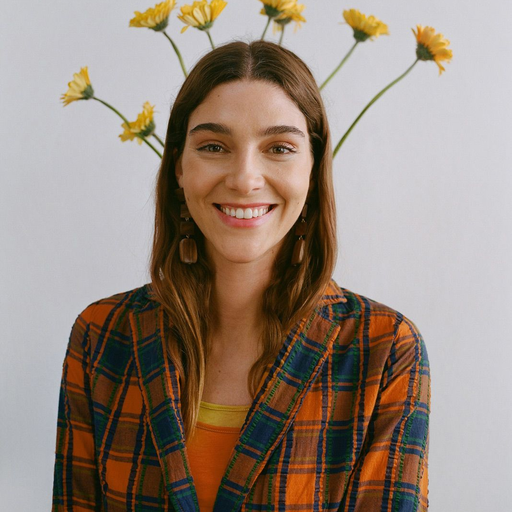
\includegraphics[width=\iw cm]{original.png}};
\node[inner sep=0pt, anchor=north west] (imgd) at (15.25,5.55) {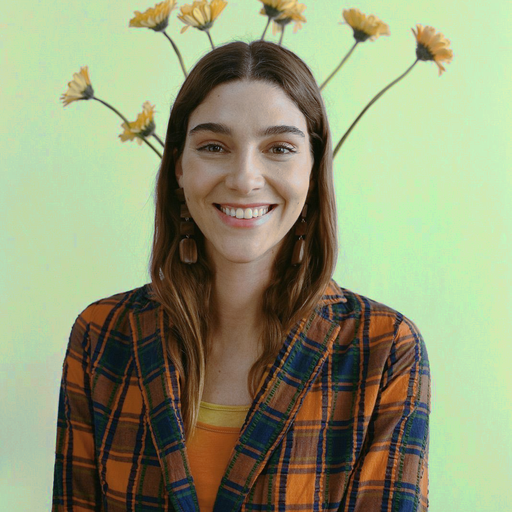
\includegraphics[width=\iw cm]{protected.png}};
\draw[black!50, line width=0.4pt] (imgx.south west) rectangle (imgx.north east);
\draw[ours, line width=0.8pt] (imgd.south west) rectangle (imgd.north east);
\node[lab, above] at (imgx.north) {$x$};
\node[lab, above] at (imgd.north) {$\tilde{x}$};
\draw[->, ours, line width=1pt] (imgx.east) -- (imgd.west) node[lab, midway, above, text=ours] {$T_\Theta$};

% 同色像素 → 同一個 c → c′
\coordinate (pa) at ($(imgx.north west)+(228/512*\iw,-85/512*\iw)$);
\coordinate (pb) at ($(imgx.north west)+(423/512*\iw,-378/512*\iw)$);
\coordinate (qa) at ($(imgd.north west)+(228/512*\iw,-85/512*\iw)$);
\coordinate (qb) at ($(imgd.north west)+(423/512*\iw,-378/512*\iw)$);
\tikzset{link/.style={line width=0.75pt, preaction={draw=white, line width=1.9pt}}}
\draw[link, ink] (pa) -- (DC) (pb) -- (DC);
\draw[link, ours] (qa) .. controls (15.75,3.3) and (12.4,3.35) .. (DCP);
\draw[link, ours] (qb) .. controls (16.2,3.2) and (12.6,3.25) .. (DCP);
\pixelring{pa}{ink}\pixelring{pb}{ink}\pixelring{qa}{ours}\pixelring{qb}{ours}
\node[circle, draw=white, line width=1.6pt, inner sep=2.1pt] at (DC) {};
\node[circle, draw=ink, line width=0.9pt, fill=colorc, inner sep=2.1pt] at (DC) {};
\node[circle, draw=white, line width=1.6pt, inner sep=2.1pt] at (DCP) {};
\node[circle, draw=ours, line width=0.9pt, fill=colorcp, inner sep=2.1pt] at (DCP) {};

% 凍結的編碼器與目標
\coordinate (e0) at (14.15,2.25);
\fill[black!12] ($(e0)+(-0.32,0.42)$) -- ($(e0)+(0.32,0.2)$) -- ($(e0)+(0.32,-0.2)$) -- ($(e0)+(-0.32,-0.42)$) -- cycle;
\draw[black!60, line width=0.6pt] ($(e0)+(-0.32,0.42)$) -- ($(e0)+(0.32,0.2)$) -- ($(e0)+(0.32,-0.2)$) -- ($(e0)+(-0.32,-0.42)$) -- cycle;
\node[lab] at ($(e0)+(-0.04,0)$) {$\mathcal{E}$};
\begin{scope}[shift={($(e0)+(-0.92,0.78)$)}]
  \draw[black!55, line width=0.5pt] (-0.07,0.02) arc (180:0:0.07);
  \fill[black!55] (-0.1,-0.11) rectangle (0.1,0.03);
\end{scope}
\node[small, anchor=west] at ($(e0)+(-0.79,0.78)$) {frozen VAE encoder};
\draw[flow] (imgx.south) |- ($(e0)+(-0.33,0.12)$);
\draw[flow] (imgd.south) |- ($(e0)+(0.33,0.05)$);
\node[small, anchor=south west] at ($(imgx.south |- e0)+(0.1,0.14)$) {$\mu_{\mathcal{E}}(x)$};
\node[small, anchor=south east] at ($(imgd.south |- e0)+(-0.1,0.07)$) {$\mu_{\mathcal{E}}(\tilde{x})$};
\draw[flow] ($(e0)+(0,-0.43)$) -- ($(e0)+(0,-0.72)$);
\node[lab, anchor=north] (obj) at ($(e0)+(0.35,-0.74)$) {$\max_\Theta\ \tfrac{1}{n}\big\|\mu_{\mathcal{E}}(\tilde{x})-\mu_{\mathcal{E}}(x)\big\|_2^2$};
\node[small, anchor=north] at ($(obj.south)+(0,0.04)$) {no instruction};
\draw[grad] (obj.west) -- ++(-0.4,0) node[lab, left, text=ours] {$\nabla_\Theta$ to (a)};
\end{tikzpicture}
\end{document}
